\chapter{Content Analysis}

Content analysis is a technique deployed by information architects for helping
them generate a sound and well structured website architecture. It consists of
two phases: collection of a representative sample of data and an analysis of
this content \citep[pp.~241--243]{morville06}.
A graphical content mapping can be included as an optional
intermediate phase between data inventory and analysis if one finds such
representations helpful for understanding a website's structure.
In it's essence a content analysis should identify the various
relationships (or lack of correlation) between a website's content items.
% all references needed

Instead of using content analysis as a means for improving on an existing
site's content architecture we'll be tailoring this technique to best help us
discover and understand social navigation patterns in infamous websites which
are known to make good use of such navigational designs. This means that we'll
concentrate only on core content objects and the relationships amongst them
which are organically generated---relationships which are made as part of
past users' behavior which can be leveraged by other users as a social form
of navigation.

The results of the low-level content inventories can be found in
Appendix~\ref{appendix:content.inventory}
(p.~\pageref{appendix:content.inventory}).
Particularly striking % find synonym? interesting, representative, ...
samples from graphical content mappings will be sprinkled throughout the
subsequent analysis to illustrate certain findings. The content mappings in
their full glory are located in
Appendix~\ref{appendix:content.mapping}
(p.~\pageref{appendix:content.mapping}).

\section{Flickr}

Flickr is a photo sharing site which are known to be on the cutting edge when
it comes to enabling new and innovating navigational features. This subsequent
analysis of Flickr will be carried out as a registered user. One has to be
registered for interacting with the site in such a way that one leaves
persistent traces. The site has a open nature enabling anonymous access
to the majority of content.

Already on the welcome page (Figure~\ref{figure:scrsh.flickr.welcome},
p.~\pageref{figure:scrsh.flickr.welcome})
we're finding navigtion links that are social of
nature. Four thumbnails functions as sample of the most resently uploaded
photos by other members of the community. One can either navigate straight to
a detailed page for each particular photo by clicking on the respective
thumbnail (Id 6, p.~\pageref{table:flickr.content.inventory.6})
or the profile of the uploader by clicking on their user
name (Id 7, p.~\pageref{table:flickr.content.inventory.7}). Such thumbnails
with minimal meta data (the uploader) are prevelent all over Flickr as can be
seen in
Table~\ref{table:flickr.thumbnail.usage}
(p.~\pageref{table:flickr.thumbnail.usage})

\begin{table}
  \centering
  \strictpagechecktrue
  \begin{adjustwidth*}{0em}{-\wholemargin}
    \caption{Thumbnail Usage on Flickr}
    \label{table:flickr.thumbnail.usage}

    \begin{center}
      \begin{tabular}{ll}

        \toprule
        Id & Context \\
        \midrule

        1.1 &
        A user's photos \\

        1.1.1.1 &
        A user's photo-set \\

        1.4.1.2 &
        A user's photos with particular tag \\

        1.6.1.1 &
        A user's photos taken on a particular date \\

        1.7.1 &
        A user's favorite photos \\

        1.8.1 &
        A user's popular photos by interestingness \\

        1.8.2.1 &
        A user's popular photos by views \\

        1.8.3.1 &
        A user's popular photos by favorites \\

        1.8.4.1 &
        A user's popular photos by comments \\

        3.1 &
        A user's contact's photos \\

        4.1.2.1 &
        A group's pool of photos \\

        5.1 &
        All highligted photos \\

        5.3.1 &
        All interesting photos the last 7 days \\

        5.4.1 &
        All interesting photos for a particular date \\

        5.6.1.1.1 &
        All photos tagged with a particular tag \\

        5.6.1.2.1 &
        Sample of  photos within a particular cluster of tags \\

        5.6.1.2.4.1 &
        All photos within a particular cluster of tags \\

        5.6.1.3 &
        Sample of photos tagged with a particular tag \\

        5.7.1.1.1 &
        All photos taken with a particular camera model \\

        5.8.1 &
        All recent uploaded photos \\

        5.8.4.1 &
        All recent uploaded Creative Commons licenced photos \\

        5.8.4.3.1 &
        All recent uploaded photos licenced under a particular Creative
        Commons licence \\

        5.10.1 &
        All interesting photos uploaded a year ago \\

        5.11 &
        Sample of interesting photos uploaded a year ago \\

        5.14.1 &
        Sample of photos from an interesting set \\




        6 &
        Welcome page \\

        \bottomrule

      \end{tabular}
    \end{center}
  \end{adjustwidth*}
\end{table}

\begin{figure}
  \centering
  \strictpagechecktrue
  \begin{adjustwidth*}{0em}{-\wholemargin}
    \begin{minipage}[t]{0.475\wholewidth}
      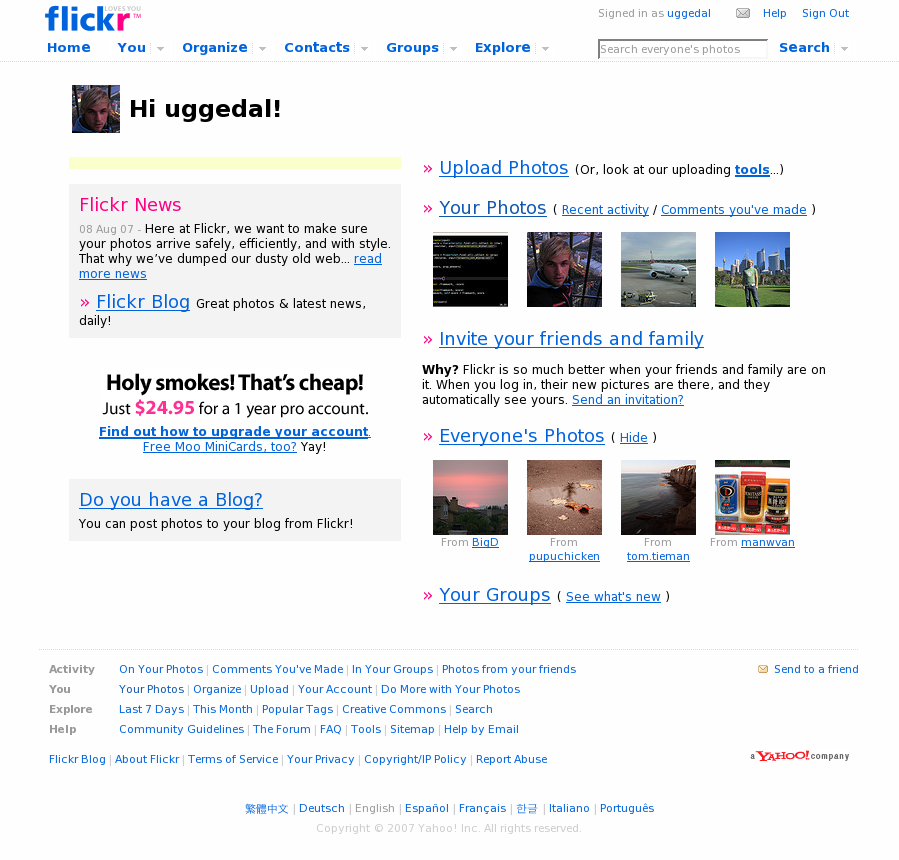
\includegraphics[width=1\textwidth]{scrsh_flickr_welcome}
      \caption[Flickr Welcome Page]{%
         The Welcome Page of Flickr
         Retrieved from the Flickr web site:
        \url{http://flickr.com/}.}
      \label{figure:scrsh.flickr.welcome}
    \end{minipage}
    \hfill
    \begin{minipage}[t]{0.475\wholewidth}
      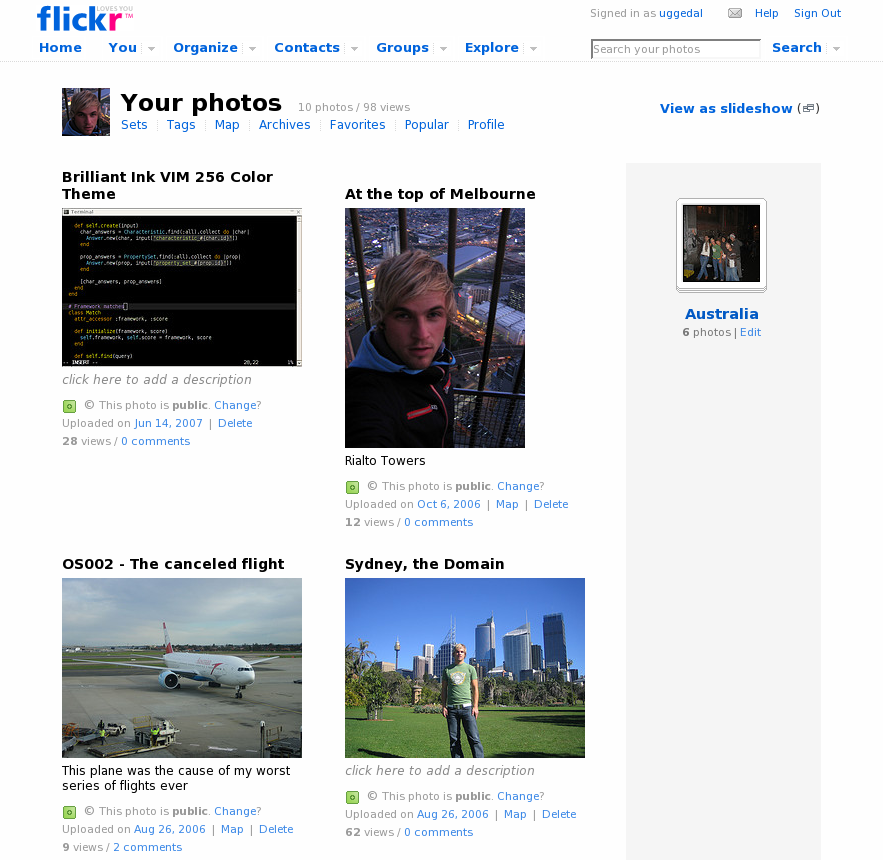
\includegraphics[width=1\textwidth]{scrsh_flickr_photos}
      \caption[Flickr Photo Page]{%
         A Photo Page from Flickr
         Retrieved from the Flickr web site:
        \url{http://flickr.com/photos/uggedal}.}
      \label{figure:scrsh.flickr.photo}
    \end{minipage}
  \end{adjustwidth*}
\end{figure}
